\chapter[The \mchem Program Package]{The \protect
\includegraphics[height=34pt]{Pics/MEGALOCHEM.pdf} Program Package}

%\begin{figure*}[h]
%\centering
%
\includegraphics[scale=1.0]{Pics/MEGALOCHEM}
%\end{figure*}

\mchem{} is a quantum chemistry program that specializes in and provides tools for low scaling electronic structure methods for ground and excited states in the atomic and local molecular orbital basis. It is  MPI parallel and can use GPUs for accelerating sparse matrix multiplication and tensor contractions via the DBCSR library. It is open-source and available on GitHub (\url{github.com/ambmax00/megalochem}). This chapter will give an overview on the software architecture and features of \mchem{}. As the program is still in development at the moment of writing, details are subject to change, and the reader is referred to the online documentation for the up-to-date user and developer guides.

\section{Motivation}

Nowadays, quantum chemists have access to a healthy ecosystem of open-source quantum chemistry programs that are under active development, including, but not limited to, CP2K \cite{Hut2014}, Dalton \cite{Aid2014}, GAMESS \cite{Gor2005}, NWChem \cite{Val2010}, Psi4 \cite{Tur2012}, PySCF \cite{Sun2018} or VeloxChem \cite{Rin2020}. They offer efficient algorithms for computing correlated ground and excited state properties, either with thread- or task-based parallelism. However, none of them support local correlation methods based on local molecular orbitals or atomic orbitals. The goal of \mchem{} is two-fold: (1) provide a framework for the development of local correlation methods and (2) offer a set of kernels for accelerating Hartree-Fock, MP2 and ADC(2) calculations, using MPI parallelism. While \mchem{} is stand-alone, it should be primarily seen as an external library or module. Quantum chemistry software packages are often composed of many different, often quite sophisticated libraries that handle e.g. evaluation of electron integrals, computation of the coulomb and exchange matrix or solving the eigenvalue problem of excited state methods. Modules allow teams of developers to concentrate on the optimization of specific libraries, rather than a whole program suite. %The ADC-connect (adcc) framework \cite{} is a good example of a highly modular library. 

\section{Software Architecture}

\mchem{} is written in C++17 and Fortran. Figure \ref{fig:MEGAARCH} shows a rough outline of its structure and dependencies. Its work flow is identical to other quantum chemistry software. An input file containing job information is parsed by the program and passed to  a driver or scheduler which sets up a series of calculations, most often in the order Hartree-Fock $\rightarrow$ Correlated Methods $\rightarrow$ Properties. The results are collected and saved to an output file.

\mchem{} takes two inputs: a \texttt{.json} file which contains the requested jobs, and an optional \texttt{.hdf5} file which contains information of the wave function from previous calculations. HDF5 (hierarchical data format) is a high-performance library and file format for storing and managing data. Data sets are organized into a filesystem-like format, called \emph{groups}, and can be accessed with a similar syntax \texttt{/path/to/dataset}. The  HDF5 library is written in C, but has bindings for C++, Fortran, Python and Java, among others. HDF5 files can also be opened and edited using external programs like HDFview or Vitables. The support for multiple languages and the simple user interface allows to easily extract information from the output file without the need to write complex bash scripts, especially for matrices like the HF coefficients, or the ADC transition matrices.  

The JSON format was chosen as the data format for the job control input, because it is a well known file format that is easy to read and edit, with multiple open-source parser libraries already available. \mchem{} has an object-oriented approach for setting up jobs, and examples of input files will be shown in section \ref{sec:JSON}.

After parsing the JSON input file and optionally loading data from previous calculations, the main driver sets up the jobs in a queue. The queue can contain multiple jobs of the same type, e.g. Hartree-Fock, with different systems and options. After initializing the parallel runtime environment, the queue is worked off and the job information is passed to the different subdrivers. \mchem{} currently has four different job types it can handle: Hartree Fock and MP2 ground state calculations, excited state calculations (CIS and ADC(2)), as well as orbital localization, analysis and plotting. Subdrivers like MP2 or ADC can read information from previous calculations, meaning that the HF wave function does not need to be recomputed each time. Output is written to \texttt{stdout} and a new HDF5 file. 

The subdrivers depend on other modules for handling evaluation of electron integrals, linear algebra and sparse matrix multiplication. 

Integrals are computed using the \texttt{libcint} library \cite{Sun2015}, which is also used in PySCF. Alternatively another branch of libcint called \texttt{qcint} may be used, that is optimized against AVX, AVX2 and AVX512. It provides the same API as libcint and no modifications to \mchem{} are necessary. However, other integral libraries can be easily swapped in. \mchem{} has its own data structures for molecules, basis sets and a general interface for requesting and handling electron integrals. Only two files need to be modified to accommodate other libraries. 

Linear algebra, such as eigenvalue decomposition, singular value decomposition and other dense matrix operations are mainly handled by the ScaLAPACK library. ScaLAPACK is written in Fortran, but \mchem{} provides C and C++ bindings for it. For node-local matrix operations, the Eigen library is used as well. 

The most crucial part of \mchem{} are the \emph{kernels}, which construct the coulomb, exchange and $Z$ matrices (encountered in AO-SOS-MP2), and compute the CIS and ADC(2) matrix vector products. Sparse matrix multiplication in the kernels is managed by the DBCSR library. \mchem{} provides an extended C++ interface (DBCSRX) with additional capabilities for ease of use. 

\begin{figure}
\centering
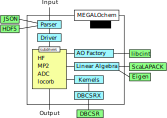
\includegraphics[scale=0.8]{Pics/megasoft}
\caption{Software architecture of the \mchem{} program package with external dependencies.}
\label{fig:MEGAARCH}
\end{figure}

\section{Parallel Runtime Environment}

As mentioned in the introduction, \mchem{} is MPI parallel. Calculations are launched using the command \texttt{mpirun}, \texttt{mpiexec} or similar. For example, the command
\begin{code}
mpirun -n 64 bin/chem h2o /scratch
\end{code}
\noindent launches 64 MPI processes with the input file \texttt{h2o.json} located in the directory \texttt{/scratch}. Process are arranged in a Cartesian grid. It is therefore crucial to choose a square number of processes for optimal performance, even if some cores on the nodes might be idle. For example, for three nodes with 24 cores each, it is better to run 64 processes instead of 72, as the performance penalty for idling cores is not significant. 

Most of the considerations for performance are dictated by the DBCSR library. DBCSR supports OpenMP parallelism, meaning a hybrid MPI+OpenMP approach is also possible for \mchem{}. However, the tensor module of DBCSR has optimal performance for 1 OpenMP thread per MPI process. The reasons are two-fold: first, each process can only allocate approximately 2.1 GB at once, which means that a larger number of MPI processes per node reduces the possibility of crashes for memory-intensive calculations. Second, not every task in the tensor library is parallelized with OpenMP threads. For these reasons, \mchem{} was also not optimized for a lower number of MPI processes, and the 1-OpenMP-thread rule is also valid for the rest of the program modules. This preference for pure MPI might conflict with other quantum chemistry software with a hybrid MPI+OpenMP approach. For more information on MPI binding and mapping, the reader is referred to the CP2K documentation, which also uses DBCSR (\url{https://xconfigure.readthedocs.io/en/latest/cp2k/#running-cp2k}).

Besides the DBCSR runtime environment, ScaLAPACK also works best with a square process grid. \mchem{} uses two separate grid instances for DBCSR and ScaLAPACK to avoid conflicts during message passing.

\section{JSON Interface \label{sec:JSON}}

Job control is specified by an input file in the JSON format. It is inspired by the BAGLE quantum chemistry software \cite{Shi2018} and follows a similar scheme to the object-oriented python interfaces like Psi4 or PySCF. Consider the following example for running a Hartree-Fock calculation on a water molecule with the cc-pVDZ basis set
\begin{code}
{
  "megalochem": [
  {
    "type": "atoms",
    "tag": "xyz",
    "unit": "angstrom",
    "geometry": [
      0.00000,        0.00000,        0.11779,
      0.00000,        0.75545,       -0.47116,
      0.00000,       -0.75545,       -0.47116
    ],
    "symbols": ["O", "H", "H"]
  },
  {
    "type": "basis",
    "atoms": "xyz",
    "tag": "basis1",
    "name": "cc-pvdz"
  },
  {
    "type": "molecule",
    "tag": "mol",
    "atoms": "xyz",
    "basis": "basis1",
    "mult": 1,
    "charge": 0
  },
  {
    "type": "hfwfn",
    "tag": "hfwfn",
    "molecule": "mol",
    "guess": "SAD",
    "build_J": "exact",
    "build_K": "exact"
   }]
}
\end{code}  
\noindent The JSON file contains a main structure \texttt{megalochem} which specifies an ordered array of objects. Each object must contain the fields \texttt{type} and  \texttt{tag}. The entry \texttt{type} specifies what kind of object it is, and \texttt{tag} is a user-defined name to uniquely define that object. This is similar to declaring a variable in a programming language. The available types are
\begin{itemize}
\item \texttt{global}: Specifies global variables like block thresholds or damping factors for electron integrals

\item \texttt{atoms}: Specifies the atomic structure of the system. It can either contain an array with coordinates or reference an XYZ file

\item \texttt{basis}: Specifies the basis set and what kind of clustering is used. Clustering indicates how atomic orbitals are grouped into blocks. A cutoff parameter can also be specified for removing linear dependencies

\item \texttt{molecule}: Specifies molecular information like multiplicity and charge

\item \texttt{hfwfn}: Job control for computing the HF wave function

\item \texttt{mpwfn}: Job control for computing the MP2 wave function

\item \texttt{adcwfn}: Job control for computing CIS and ADC(2) excitation energies

\item \texttt{moprint}: Job control for localizing and plotting orbitals (CMOs, LMOs, NTOs) from different calculations

\end{itemize} 

\noindent Some objects may reference other preceding objects. For example, the \texttt{adcwfn} object needs to reference a \texttt{hfwfn} object on which to operate.

This object-oriented approach will also facilitate a potential implementation of a python interface to \mchem{}.

\section{Design Patterns}

One of the major challenges in designing a modular quantum chemistry software is deciding how arguments are passed from one module to another. Implementations of electronic structure methods often accept dozens of different keywords, leading to complex function and constructor signatures, and grouping keywords into logical structures is non-trivial. A popular solution to this problem is the use of a \texttt{options} class which group parameters into an overarching \emph{context}, such as \texttt{psi4::options} in Psi4 or \texttt{libctx::context} in Q-Chem. The advantage is that keywords are easily accessed by requesting it by name. Existence of the keys can also be checked by using member functions. However, this is at the same time the greatest downside of context classes. For a complex hierarchy of interacting modules and functions, which can all insert or delete keywords, it is often impossible to know what  objects are or are not present within the context at a given level. 

Contexts are therefore not used in \mchem{}. This leads to more verbose code, as each class needs to explicitly define all its parameters, but it is less error-prone. Optional parameters are handled using a modified \texttt{std::optional} class.

Large classes are constructed using the \emph{factory method pattern} and parameters are passed to the factory class by calling a chain of \emph{setter} member functions. Consider the following example for defining a Hartree-Fock object:
\begin{cppinline}
auto hfobj = hf::hfmod::create()				 
 .set_world(my_world)
 .set_molecule(my_molecule)
 .df_basis(dfbas) 
 .build_J("dfao") // optional
 .build_K("dfao") // optional
 .guess("SAD")    // optional
 .build();
\end{cppinline}
\noindent It sets up a density-fitting calculation of a Hartree-Fock wave function. Objects like \texttt{world} and \texttt{molecule} are required, and will give a runtime error if they are not set before calling \texttt{build()}. Other parameters are optional, and can either be set or just omitted. The factory function pattern needs a lot of boiler-plate code, but imposing the pattern is facilitated by the use of preprocessor directives. Each module header file has a preprocessor list of required and optional parameters before the class definition. For the \texttt{hfmod} class, it reads
\begin{cppinline}
#define HFMOD_LIST \
  (((world), set_world), 
   ((desc::shared_molecule), set_molecule), \
   // ... other parameters
  )
#define HFMOD_LIST_OPT \
  (((util::optional<std::string>), guess, "SAD"), \
   ((util::optional<double>), scf_threshold, 1e-6), \
   ((util::optional<int>), max_iter, 100), \
   ((util::optional<bool>), do_diis, true), \
   ((util::optional<int>), diis_max_vecs, 10), \
   ((util::optional<int>), diis_min_vecs, 2), \
   ((util::optional<int>), diis_start, 1), \
   ((util::optional<std::string>), build_J, "exact"), \
   ((util::optional<std::string>), build_K, "exact"), \
   ((util::optional<std::string>), df_metric, "coulomb"), \
   // ... other parameters
   )
\end{cppinline}

\noindent New keywords can be easily added to the list. For optional parameters, there is also the possibility to add default values. The lists are then passed to preprocessor functions which automatically generate the necessary code for the factory functions. They construct a \texttt{struct} containing all of the parameters in the list which can be used in the constructor of the module class. While this approach is more verbose, it provides a clearer overview of possible input parameters. 

\section{Libraries \label{sec:LIBS}}

This section provides an overview of the different modules present in \mchem{}, and presents some examples on how to use them. 

All information on the parallel MPI runtime environment, that is, communicators and Cartesian grids for the DBCSR and ScaLAPACK libraries, are stored in a class called \texttt{megalochem::world}. It contains information on the rank, size and topology of the different grids. 

\subsection{\texttt{dbcsrx}}

The \texttt{dbcsrx} module is an extended C++ interface to the DBCSR library. Most objects are constructed using the factory function pattern explained in the previous section. Classes may have different constructors with a different set of keywords. Matrices are easily constructed from scratch by using the \texttt{create} function
\begin{cppinline}
std::vector<int> blksizes = {2,5,6,3};
dbcsr::shared_matrix<double> 
my_matrix = dbcsr::matrix<>::create()
	.set_cart(world.dbcsr_grid())
	.name("My Matrix")
	.row_blk_sizes(blksizes)
	.col_blk_sizes(blksizes)
	.matrix_type(dbcsr::type::symmetric)
	.build();
\end{cppinline}
\noindent which returns a \texttt{std::shared\_ptr} to a dbcsr matrix object, or \texttt{dbcsr::shared\_matrix} for short. In general, all the factory functions return pointers rather than objects. The matrix class needs the Cartesian grids, row and column block sizes, as well as the matrix type (symmetric, hermitian, nonsymmetric, ...). Factory functions can also be used to construct copies of the matrix, e.g.
\begin{cppinline}
auto my_copy = dbcsr::matrix<>::copy(*my_matrix)
	.name("My Copy")
	.build();
\end{cppinline}
\noindent There are further factory functions for constructing templates, transposes or reading data from disk.

Tensors are constructed in a similar way, but additionally need a \texttt{pgrid<N>} (process grid) object which is a $N$-dimensional general Cartesian grid. The underlying matrix representation also needs mapping information (see previous chapter). A tensor can then be allocated by
\begin{cppinline}
std::array<std::vector<int>,3> 
arrvec = {blksizes1, blksizes2, blksizes3};

dbcsr::shared_pgrid<3> 
my_pgrid = dbcsr::pgrid<3>::create(world.comm()).build();

dbcsr::shared_tensor<3>
my_tensor = dbcsr::tensor<3>::create()
	.set_pgrid(my_pgrid)
	.name("My Tensor")	
	.blk_sizes(arrvec)
	.map1({0}).map2({1,2})
	.build();
\end{cppinline} 

Each class has member functions which have a Fortran analog in the DBCSR library. The object-oriented C++ interface greatly reduces the complexity of the code, as the C interface of the DBCSR library can become quite unwieldy at times.

The matrix multiplication and tensor contraction functions are also used in a factory function-like manner and their function signatures resemble those of the LAPACK \texttt{gemm} routines
\begin{cppinline}
dbcsr::shared_matrix<> A, B, C;
// allocate and fill matrices ...

// perform C = 3 * A * B + C 
dbcsr::multiply('N', 'N', 3.0, *A, *B, 1.0, *C)
	.filter_eps(1e-8) // pass optional parameters 
	.perform();
\end{cppinline}
\noindent The tensor contraction routines have been extended to work with Einstein summation:
\begin{cppinline}
dbcsr::shared_tensor<3> A, C;
dbcsr::shared_tensor<4> B;
// allocate and fill ...

// perform C("ikl") = 3 * A("ljm") * B("ikjm")
dbcsr::contract(3.0, *A, *B, 0.0, *C)
	.perform("ljm, ikjm -> ikl");
\end{cppinline}
\noindent which greatly simplifies the implementation.

One of the more prominent extensions in dbcsrx is the \texttt{btensor} (batched tensor) class. Tensor contractions often need to be performed in batches for memory efficiency. This however means that the tensor needs to be split appropriately along each dimension. The \texttt{btensor} class manages the necessary metadata of batched tensor contractions and provides helper functions to the developer. Moreover, it is possible to pass a \texttt{btype} variable to the constructor which specifies whether the tensor is held in core memory, read from disk, or generated on-the-fly. The interface remains the same, irregardless of how the tensor is stored, meaning that in-core, disk and direct algorithms do not need separate implementations. Disk batched tensors store data in block-wise format on disk using MPI I/O, meaning each process can read and write independently. Direct batch tensors furthermore need a generator function that indicates how the data is generated, for example in the case of atomic orbital electron integrals. 

The \texttt{dbcsrx} module also provides several functions for converting to ScaLAPACK and Eigen matrix formats. 

\subsection{\texttt{math}}

The \texttt{math} library contains the C++ interface to the ScaLAPACK functions for matrix decompositions, as well as DIIS and Davidson solver routines, a routine for incomplete pivoted Cholesky decomposition, and an interface to the Fortran library by Helmich-Paris and Visscher \cite{Hel2016} for computing the Laplace quadrature parameters. 

The ScaLAPACK interface accepts DBCSR matrices which are then converted to the fixed block-cyclic format used by ScaLAPACK. The following example shows the eigenvalue decomposition of a hermitian matrix:
\begin{cppinline}
hermitian_eigen_solver hsolver(world, *my_matrix, 'V', true);
hsolver.compute();
auto eigenvalues = hsolver.eigvals();
auto eigenvectors = hsolver.eigvecs();
\end{cppinline} 

\subsection{\texttt{ints}}

Evaluation of electron integrals, as well as the computation of density fitting coefficients is handled by the \texttt{ints} module. The interface for requesting integrals is general and does not depend on what integral library is used. Integrals are computed by constructing an \texttt{aofactory} object
\begin{cppinline}
auto factory = ints::aofactory(my_world, my_molecule);

// get the overlap integrals
dbcsr::shared_matrix<> s_bb = factory.ao_overlap();
dbcsr::shared_matrix<> k_bb = factory.ao_kinetic();
\end{cppinline}
\noindent Computing the 3c2e and 4c2e integrals is more complex, as they need to be evaluated in batches and more information needs to be passed to the functions:
\begin{cppinline}
dbcsr::shared_tensor<3> eri_3c2e;
// allocate tensor

factory.ao_3c2e_setup(metric::coulomb);
factory.ao_3c2e_fill(eri_3c2e);
\end{cppinline}
\noindent For this reason, the user should prefer the auxiliary  \texttt{aoloader} class, where integrals are first requested, and then computed.
\begin{cppinline}
auto loader = ints::aoloader::create()
	.set_world(my_world)
	.set_molecule(my_molecule)
	.build();
	
loader.request(ints::key::s_bb)
	.request(ints::key::coul_xbb)
	.request(ints::key::dfit_coul_xbb);
	
loader.compute();
\end{cppinline}
\noindent Integrals are requested by a predefined set of keys. Fitting coefficients can also be computed by the \texttt{aoloader} class. Furthermore, it also resolves any dependencies and computes all the necessary integrals, even if they were not specifically requested. The integral library can compute the following density fitting coefficients:
\begin{itemize}
\item Standard coulomb metric
\item Coulomb-attenuated metric
\item Overlap metric
\item Quasi-robust density fitting
\item Pair-atomic resolution of the identity
\end{itemize}

\subsection{\texttt{fock}}

The \texttt{fock} library provides kernels for computing the coulomb and exchange matrix. The kernels follow the factory pattern, which returns a general \texttt{fock::J} or \texttt{fock::K} which works the same irrespective of which method is chosen to evaluate the coulomb and exchange matrices.
\begin{cppinline}
std::shared_ptr<fock::J> 
jbuilder = fock::DF_J::create()
	.set_world(my_world)
	.molecule(my_molecule)
	.eri3c2e_batches(my_tensor)
	.metric_inv(my_matrix)
	.build();
	
jbuilder->init();

// compute density matrix 
dbcsr::shared_matrix P_bb = ...
jbuilder->set_density_alpha(*P_bb);

// compute coulomb matrix
auto J_bb = jbuilder->get_J();
\end{cppinline} 
\noindent After calling \texttt{build()}, the object needs to be initialized. For each SCF cycle, the kernel is updated with the current density matrix. The matrix is then constructed by calling the \texttt{get} functions. The coulomb matrix can be computed with the kernels
\begin{itemize}
\item \texttt{EXACT}: exact coulomb matrix without density fitting
\item \texttt{DFAO}: coulomb matrix with density fitting in the AO basis
\end{itemize}
\noindent and the following kernels are available for the exchange matrix
\begin{itemize}
\item \texttt{EXACT}: exact exchange matrix without density fitting
\item \texttt{DFAO}: density fitting in the AO basis
\item \texttt{DFMO}: density fitting in the MO basis
\item \texttt{DFAOMEM}: density fitting in the AO basis, with the fitting coefficients computed on-the-fly
\item \texttt{DFROBUST}: density fitting using Dunlap's robust density fitting formula 
\end{itemize}

\noindent The \texttt{EXACT} kernels are not optimized and should only be used for reference calculations. 

\subsection{\texttt{hf}}

The \texttt{hf} module computes the Hartree-Fock wave function using the self-consistent field methods. The Fock matrix is computed with the $J$ and $K$ kernels, and different methods can be easily combined. The guess is computed either from the core Hamiltonian, the superposition of atomic densities (SAD) or projection methods (see Appendix \ref{sec:SCFGUESS}). 

\subsection{\texttt{mp}}

The \texttt{mp} library contains the kernels for computing the $Z$ matrix encountered in AO-DF-SOS-MP2. The kernels are initialized similarly to the $J$ and $K$ kernels. Two different types have been implemented 
\begin{itemize}
\item \texttt{LLMP\_FULL}: computes the Z kernel by constructing the fully transformed $B_{X\ulgm\olgn}$ tensor and keeping it in core memory
\item \texttt{LLMP\_MEM}: the tensor $B_{X\ulgm\olgn}$ is recomputed on-the-fly when contracting it with $B_{X\mu\nu}$
\end{itemize} 

\subsection{\texttt{adc}}

The final set of kernels is contained in the \texttt{adc} library, which compute the AO-CIS and CDD-DF-SOS-ADC(2) matrix-vector product and reuse the $J$, $K$ and $Z$ kernels from the other modules to evaluate some of the expressions. The \texttt{adc} library solves the ADC eigenvalue problem by using the (modified) Davidson method. Only eigenvalues can be computed at the moment.

\subsection{\texttt{locorb}}

The \texttt{locorb} module provides routines for localizing molecular orbitals. The available localization schemes are
\begin{itemize}
\item Foster-Boys LMOs 
\item Cholesky LMOs
\item Projected atomic orbitals
\end{itemize}
\noindent Furthermore, the library can compute the natural transition orbitals from the CIS or ADC(2) density matrices. The orbital information can be written to a file in \texttt{molden} format for plotting in external software. 

%\section{Installation}
%
%\subsection{Prerequisites}
%
%MEGALOchem depends on the following external libraries:
%\begin{itemize}
%\item LAPACK
%\item ScaLAPACK
%\item Eigen (header only)
%\item DBCSR, configured with LIBXSMM
%\item libcint (version 4.4.5 or higher) configurated with \texttt{WITH\_RANGE\_COULOMB=ON} and \\ \texttt{WITH\_COULOMB\_ERF=ON} to enable coulomb-attenuated metrics
%\item HDF5, with MPI enabled
%\end{itemize}
%
%\noindent Furthermore, you will need
%\begin{itemize}
%\item CMake (version 3.17+)
%\item Fortran compiler which supports the 2008 standard including the TS 29113 for C-bindings
%\item C++ compiler with c++17 standard (GCC 9.2.0+ or Intel 19.1+) and MPI support (version 4.0+)
%\end{itemize}
%
%\subsection{Build}
%
%The executable is build using cmake. Inside the megalochem directory, run
%\begin{code}
%mkdir build 
%cd build 
%cmake ..
%\end{code}
%\noindent Additional configuration flags for cmake are:
%\begin{lstlisting}[backgroundcolor=\color{light-gray},breaklines=true,basicstyle=\small\ttfamily]
%-DDBCSR_DIR = <location of DBCSR config file>
%\end{lstlisting}
%\begin{itemize}
%\item \texttt{-DDBCSR\_DIR = <location of DBCSR config file>}
%\end{itemize}
%
%\section{Features}
%
%\section{Input File}
%
%\section{Running MEGALOchem}
%
%MPI processes grid, openmp ...
%
%\begin{verbatim}
%Hi this is code
%\end{verbatim}


